\documentclass{article}

\usepackage{amssymb}
\usepackage{amsmath}
\usepackage[french]{babel}
\usepackage[utf8]{inputenc} 
\usepackage[T1, T2A]{fontenc}

\usepackage{listings}

\usepackage[a4paper,left=2cm,right=2cm,top=2cm,bottom=2cm]{geometry}

\usepackage{setspace}

\usepackage{graphicx}

\usepackage{stmaryrd}

\setlength{\parindent}{0cm}
\setlength{\parskip}{1ex plus 0.5ex minus 0.2ex}
\newcommand{\hsp}{\hspace{20pt}}
\newcommand{\HRule}{\rule{\linewidth}{0.5mm}}

\title{Compte rendu}
\author{Arthur Lacoin - Timothé Rios}

\date{}
    
\begin{document}

\begin{titlepage}
    \begin{sffamily}
    \begin{center}

        \textsc{\LARGE Lycée Lakanal}~\\[2cm]

        \HRule \\[0.4cm]
        { \huge \bfseries Simulation d'épidémies à l'aide d'automates cellulaires\\[0.4cm] }
        \HRule \\[2cm]
        \textsc{\Large Arthur Lacoin - Timothé Rios}\\[2cm]

    \end{center}
\end{sffamily}
\end{titlepage}

\tableofcontents

\newpage

\begin{center}
\textsc{Introduction}~\\[1cm]
\end{center}

	L'étude de la propagation des maladies est une science qui remonte à la Grèce Antique, lorsque Hippocrate, au quatrième siècle avant Jésus-Christ, créa les termes d'endémie et d'épidémie afin de qualifier respectivement des maladies liées à des endroits et à des périodes donnés. Mais cette science ne se développa vraiment qu'en 1854, quand John Snow, un médecin britannique, étudia la propagation de l'épidémie de choléra dans les quartiers de Londres. Ce sont là les prémices de l'épidémiologie, l'étude du transport des infections. De nos jours, les méthodes ont évolué et la méthode différentielle, que l'on présentera plus loin, est la plus fréquemment utilisée. Nous nous sommes intéressés ici à la simulation par automates cellulaires.

\section{Première version}

\subsection{Présentation}
\paragraph{Définition formelle\\[0.2cm]}
	Un automate cellulaire est une matrice de cellules, chacune ayant un état appartenant à un ensemble prédéfini. L'état de chaque cellule peut varier au cours du temps suivant une fonction de transfert : l'état de la matrice à l'instant $t+1$ dépend ainsi de son état à l'instant $t$. L'automate doit donc posséder un état initial, c'est-à-dire la matrice des états initiaux des cellules. Même si son principe de base est simple, l'automate cellulaire se complexifie grandement lorsque la taille de la grille augmente, ce qui en fait un modèle couramment utlisé dans l'étude des systèmes complexes.

\paragraph{Historique\\[0.2cm]}
	Les automates cellulaires sont plutôt récents. Ils ont été mis au point par John Von Neumann dans son étude des systèmes auto-réplicatifs dans les années 1940. Cette notion a été grandement popularisée par le "jeu de la vie" de John Conway, un automate cellulaire en deux dimensions paru dans les années 1970. À ce jour, les automates cellulaires ont de nombreuses applications dans divers domaines :
	\begin{itemize}
	\item diffusion d'un gaz en s'appuyant sur les équations de Navier-Stokes
	\item simulation des feux de forêts
	\item simulation du trafic routier
	\end{itemize}

\paragraph{Notre automate cellulaire\\[0.2cm]}
	Notre automate cellulaire est un automate en deux dimensions qui vise à simuler la propagation d'une épidémie. Les cellules ont donc un état parmi les quatre suivants : Sain, Malade, Guéri, Mort. L'état Sain est l'état initial que chaque cellule sauf une possède à la première étape de la simulation. Lorsqu'une cellule est saine, elle peut tomber malade avec une probabilité $p_1$ s'il y a des malades dans son entourage. L'état Malade est au départ donné à une seule cellule, le "patient zéro". Une cellule malade peut soit mourir avec une probabilité $p_2$ soit guérir avec une probabilité $p_3$. Les cellules mortes ou guéries restent dans cet état indéfiniment, l'hypothèse prise étant qu'une cellule guérie est immunisée et ne peut plus attraper la maladie. Enfin, la simulation s'arrête lorsqu'il n'y a plus de cellule malade, car l'état de l'automate ne peut alors plus varier.
	
\paragraph{Calcul des probabilités\\[0.2cm]}
	Les probabilités d'infection, de soin et de mort que nous avons utilisé ont été calculées à partir de paramètres empiriques tirés d'études réelles. On utilisera en particulier $\tau$, le temps moyen qu'un individu reste infecté, et $R_0$, le nombre moyen d'individus qu'un malade contamine durant son temps de contamination.
	
	On cherche d'abord à déterminer la probabilité d'infection. On se place donc dans $(\Omega, P)$ un espace probabilisé fini. On étudie un individu malade entouré de $n$ voisins sains. On considère que l'infection d'un individu sain est indépendante des autres. \\
	On établira d'abord un résultat préliminaire.\\
	Soit $X, Y$ deux variables aléatoires réelles sur $\Omega$ et à valeur dans $\llbracket 0, n \rrbracket, n \in \mathbb{N}$, telles que $\forall k \in \llbracket 0, n \rrbracket, X$ sachant que $Y = k$ suit une loi binomiale de paramètres $(n-k, p), p \in \left]0, 1\right[$.\\ \underline{Alors $E(X) = (n - E(Y))p$.}\\[0.2cm]
	On a donc $\forall k \in \llbracket 0, n \rrbracket, E_{\{Y = k\}}(X) = (n - k)p$. Par formule de l'espérance totale, 
	\begin{align*}
	E(X) &= \sum_{k=0}^n P(Y = k)E_{\{Y = k\}}(X)  \\
	     &= \sum_{k=0}^n P(Y=k)(n-k)p \\
		 &= np\sum_{k=0}^n P(Y = k) - p\sum_{k=0}^n kP(Y=k) \\
		 &= np - pE(Y) \\
		 &= p(n - E(Y))
	\end{align*}
	Soit $k \in \llbracket 1, \tau \rrbracket, X_k$ est la variable aléatoire donnant le nombre d'individus qui ont été infectés au jour $k$.\\
	$X_1 \hookrightarrow B(n, p)$ car on infecte les individus indépendamment.\\ 
	Au jour $k$ il reste $$n - \sum_{i = 0}^{k-1} X_i$$ individus sains.\\[0.2cm] \underline{Montrons par récurrence que $\forall k \in \llbracket 1, \tau \rrbracket, E(X_k) = n(1-p)^{k-1}p$}\\[0.2cm]
	
	\underline{$\forall k \in \llbracket 1, \tau \rrbracket$, notons $P(k) = "\forall i \in \llbracket 1, k \rrbracket, E(X_i) = n(1-p)^{i-1}p"$}.\\[0.2cm]
	\underline{$P(1)$ est vraie} car $X_1 \hookrightarrow B(n, p)$.\\[0.2cm]
	\underline{Ou bien $\tau = 1$} et c'est fini.\\[0.2cm]
	\underline{Ou bien $\tau \ge 2$} et on \underline{suppose que $P(k)$ est vraie pour $k \in \llbracket 1, \tau - 1 \rrbracket$. Montrons que $P(k+1)$ est vraie.}\\[0.2cm]
	$\forall i \in \llbracket 1, k \rrbracket, E(X_i) = n(1-p)^{i-1}p$ par $P(k)$. Il reste à calculer $E(X_{k+1})$.\\
	\begin{align*}
		E(X_{k+1}) &= p(n - \sum_{i = 1}^n E(X_i)) \\
		           &= p(n - \sum_{i = 1}^n n(1-p)^{i - 1}p \\
		           &= np(1-p)^k
	\end{align*}
	On conclut par récurrence multiple finie.\\
	Armés de ces résultats, nous pouvons quasiment calculer $p$, car on a le nombre moyen d'infectés par un malade au cours de sa période d'infection, $R_0$. On a donc 
	\begin{align*}
		R_0 &= \sum_{k=1}^\tau E(X_k) \\
		    &= \sum_{k=1}^\tau np(1-p)^{k-1}\\
		    &= np\frac{1 - (1-p)^\tau}{p}\\
		    &= n(1 - (1-p)^\tau)
	\end{align*}
	
	Ce qui nous amène par de brefs calculs à la conclusion : \\
	$$p = 1 - \sqrt[\tau]{\frac{n - R_0}{n}}$$.\\
	
	On cherchera désormais à calculer la probabilité de ne plus être malade, c'est à dire ou bien de guérir ou bien de mourir, c'est à dire $p_{\text{mort}} + p_{\text{guérison}} = q$. Si l'on considère un individu qui est infecté au jour $0$, et que l'on considère la variable aléatoire $X$ donnant le jour de guérison(sachant qu'on ne peut guérir le jour de son infection), $\forall k \in \mathbb{N}^*, P(X=k) = (1-q)^{k-1}q$.\\
	X suit donc une loi géométrique et son espérance, c'est à dire le nombre de jour où l'individu restera malade($\tau$) vaut par propriété $\frac{1}{q}$.\\
	On a donc $$ q = \frac{1}{\tau}$$\\
	

Enfin pour calculer la probabilité de mourir, il suffit de faire $mq$, où $m$ est la mortalité de la maladie, et la probabilité de guérir vaut $(1-m)q$. \\
Les résultats réels sont récapitulés dans le tableau suivant :

\begin{tabular} {| p{2cm} | p{2cm}| p{2cm} | p{2cm} |}
	\hline
	Maladie & $p_{infection}$ & $p_{mort}$ & $p_{guerison}$ \\ \hline
	Ebola & $0.0201$ & $0.0818$ & $0.00909$ \\
	\hline
\end{tabular}

\subsection{Résultats}

Voici quelques étapes d'une simulation de notre automate. Le foyer originel -la première cellule infectée- est placée au centre de la grille à l'étape 1. Sur ces images,représentant la grille de l'automate, les cellules saines sont représentées en blanc, celles malades sont rouges, celle guéries sont vertes et celles mortes sont noires.

\begin{figure}[hbtp]
\centering
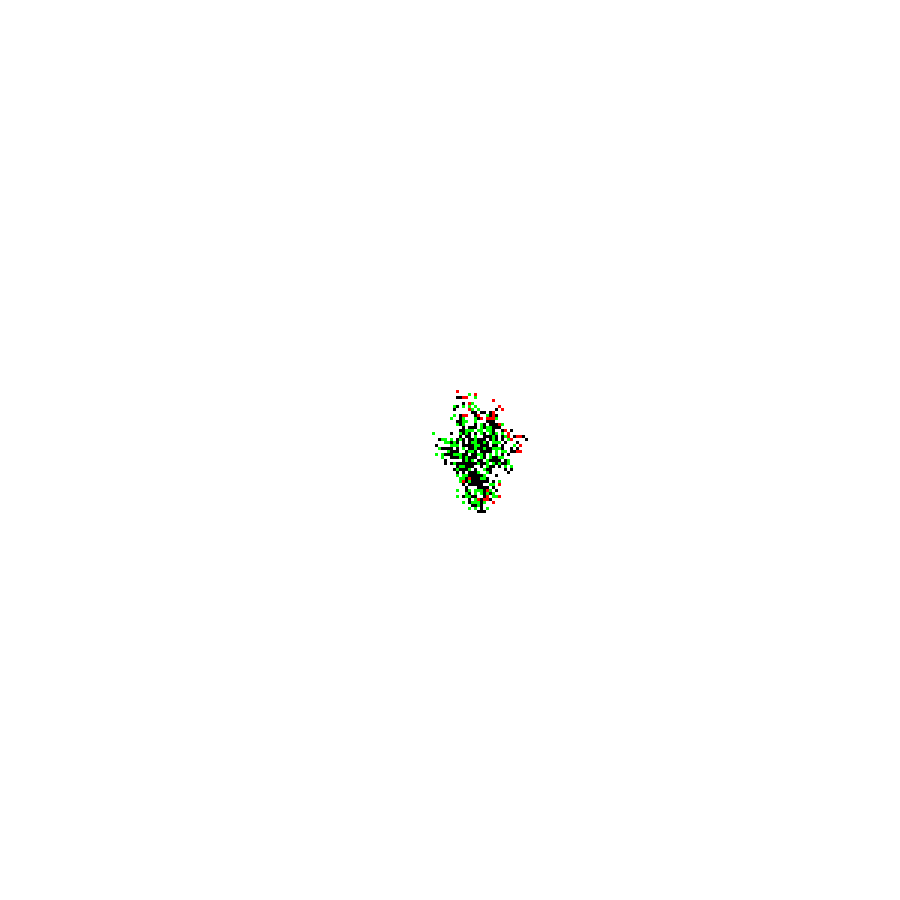
\includegraphics[scale=0.22]{Frame-36.png}
\caption{Étape 36}
\end{figure}

\begin{figure}[hbtp]
\centering
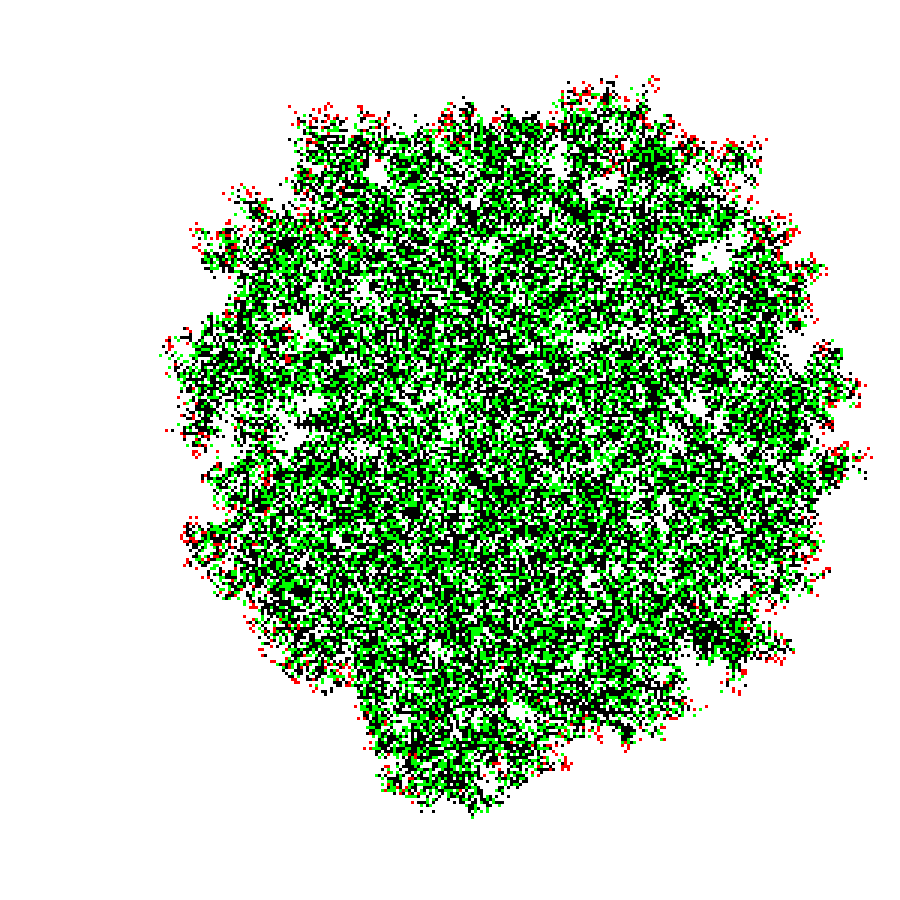
\includegraphics[scale=0.22]{Frame-195.png}
\caption{Étape 195}
\end{figure}

\begin{figure}[hbtp]
\centering
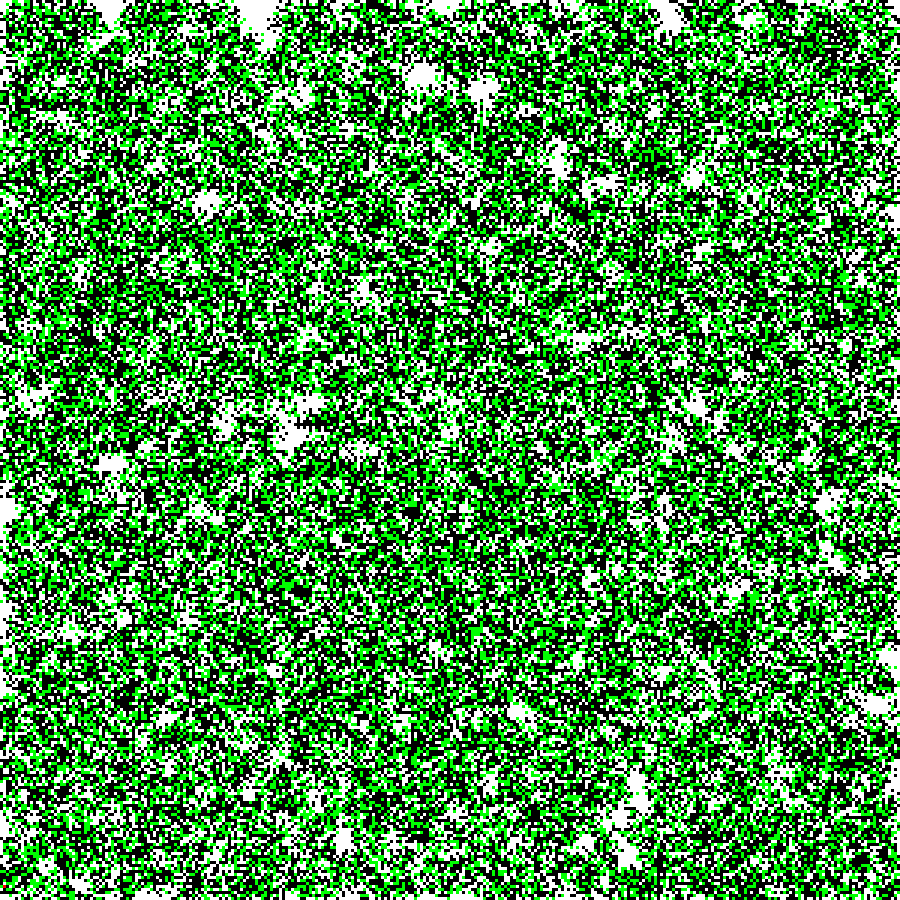
\includegraphics[scale=0.22]{Frame-412.png}
\caption{Étape 412}
\end{figure}





Dans la simulation présentée ci-dessous, les probabilités d'infection, de guérison et de mort ont été choisies arbitrairement afin de procurer un visuel clair du comportement de l'automate. Voici encore d'autres exemples de cas possibles de comportements de maladie, dont l'évolution est cette fois-ci représentée sur un graphique donnant le nombre de personnes saines, malades, guéries et mortes au cours des étapes de la simulation.



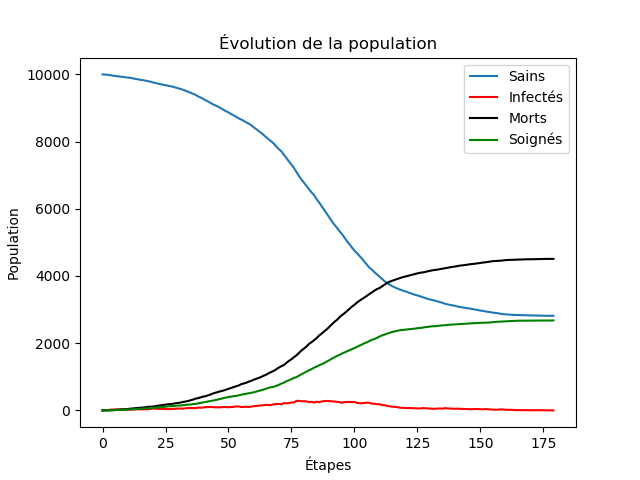
\includegraphics[scale=1]{g.png} 


	Dans ce cas, $p_1$ valait 0.2, $p_2$ valait 0.25, $p_3$ valait 0.2 et la maladie pouvait se transmettre dans un rayon de deux cellules autour de l'infectée.

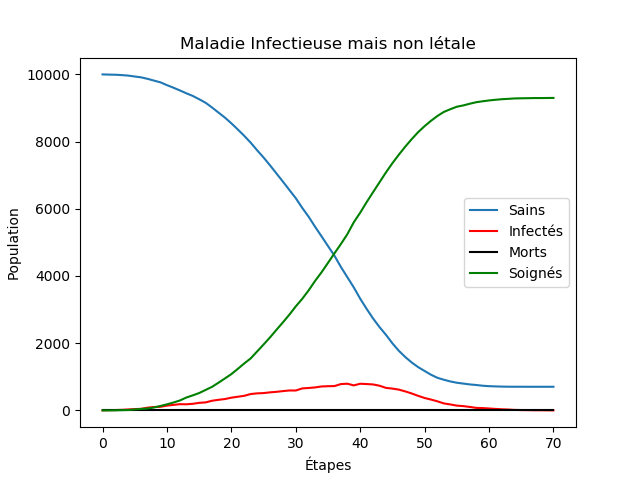
\includegraphics[scale=1]{Figure_2.png}


	Ici, nous pouvons voir l'exemple d'une maladie non létale, se rapprochant d'un rhume tout en étant bien plus infectieuse.


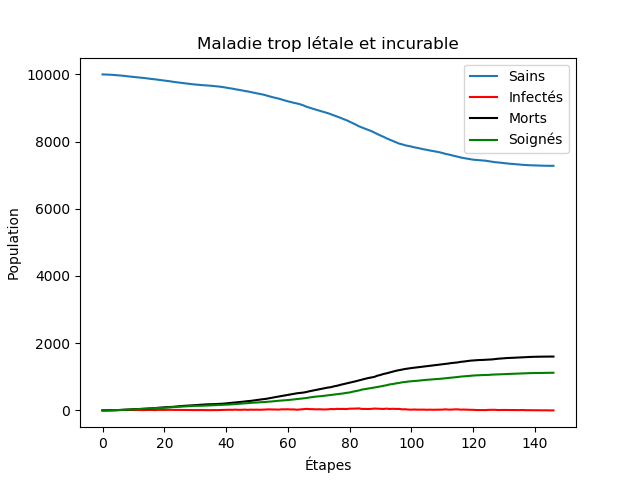
\includegraphics[scale=1]{Figure_3.png}



Dans cet exemple, la maladie est trop létale pour pouvoir se propager longtemps : les infectés meurent sans avoir eu le temps de contaminer un de leurs voisins.
\subsection{Limites}
	Cette version de l'automate cellulaire fournit déjà des résultats intéressants. Cependant, le modèle reste trop simple pour pouvoir modéliser la réalité d'une épidémie. En effet, il est ici supposé que les individus de la population étudiée restent sur place tout en étant étroitement collés les uns aux autres.
Il apparaît ainsi qu'un grand nombre de paramètres a été négligé : il est ici supposé que la population est uniformément répartie, alors qu'en réalité cette densité dépend d'un nombre important de facteurs, comme le type de terrain, les constructions humaines (villes par exemple) ou les conditions météorologiques. De plus, nous supposons aussi que l'épidémie se déroule en un temps assez court pour que les décès naturels et les naissances soient négligeables, tout comme nous négligeons les mesures que pourraient prendre certains gouvernements en cas de pandémies majeures.
	
	
	
\section{Deuxième version}

\subsection{Présentation}
	Ce deuxième automate prend en compte plus de paramètre : 
	\begin{itemize}
	\item nous avons cette fois considéré les cellules comme des zones géographiques plutôt que des individus, ayant une population ainsi qu'une répartition Sains-Malades-Morts-Guéris propre.
	\item nous avons pris en compte les densités de population, celles-ci dépendant du 'type' de case, à savoir Ville, Campagne, Montagnes ou Route.
	\item nous avons pris en compte les mouvements de population, en fonction de deux paramètres : la probabilité qu'une partie de population quitte une case, et la probabilité qu'une case a d'attirer la population des cases adjacentes.
	\end{itemize}
	
	Ces ajouts de paramètres permettent une simulation plus fine et plus proche de la réalité. Cela permet d'utiliser de bien meilleure façon les automates cellulaires, qui ont pour avantage de prendre en compte les paramètres géographiques de la simulation.


\subsection{Résultats}

Les résultats graphiques de cet automate permettent d'afficher la densité de population des quatre états au sein de toutes les cellules de la grille. Bien sûr, il n'est maintenant plus possible d'afficher tous les paramètres de la grille sur une seule image. Voici par exemple la répartition des individus sains sur une grille \\[0.6cm]


\includegraphics[scale=2]{../images/Frame-1.png} 

\includegraphics[scale=2]{../images/Frame-58.png} 

\includegraphics[scale=2]{../images/Frame-221.png}


Ici, plus une cellule contient de personnes saines, plus le pixel la représentant sur l'image est blanc. Les cellules sont donc toutes légèrement grisées à la première étape, non pas parce qu'elles contiennent des individus malades, morts ou guéris, mais parce que le programme étalonne automatiquement les couleurs en fonction de la taille de la grille et de sa population afin de pouvoir intensifier la couleur si la population saine d'une cellule augmente.
Bien sûr, cette simulation servant d'exemple pour présenter ce nouvel automate, ses cellules possèdent des probabilités de déplacement des populations bien plus élevées que dans la réalité.
On remarque dans la dernière image que l'épidémie a complètement envahie le côté droit avant les coins de gauche. Cet état est bien dû à l'incertitude causée par les probabilités.
 \subsection{Comparaison}
Ce nouvel automate nous permet donc une modélisation plus précise de l'évolution d'une maladie. Ainsi, nous avons pu comparer nos résultats,comme celui ci-dessous, avec ceux de précédentes études.

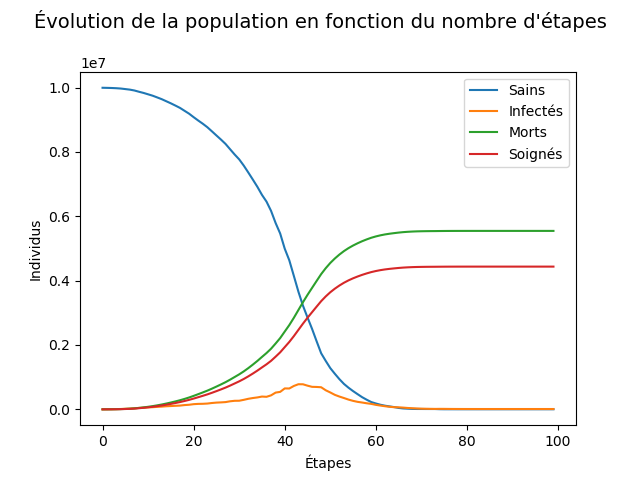
\includegraphics[scale=1]{../images/tttt.png}

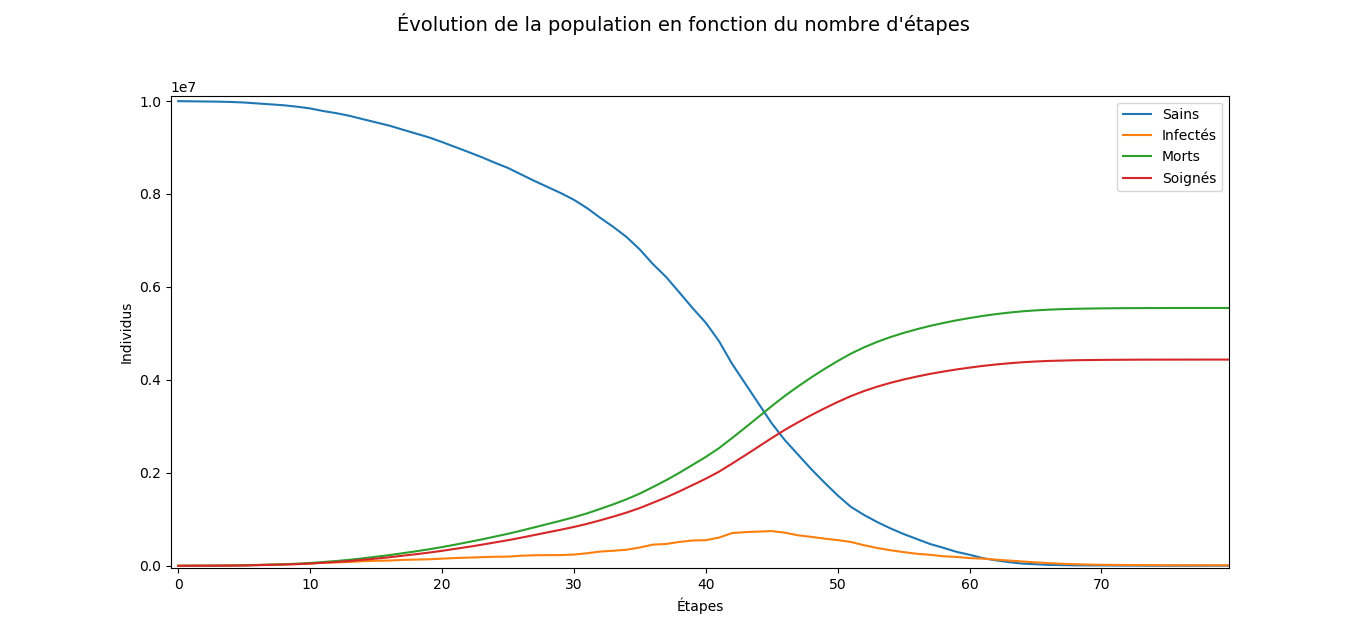
\includegraphics[scale=0.5]{../images/tttttttttt.png}   

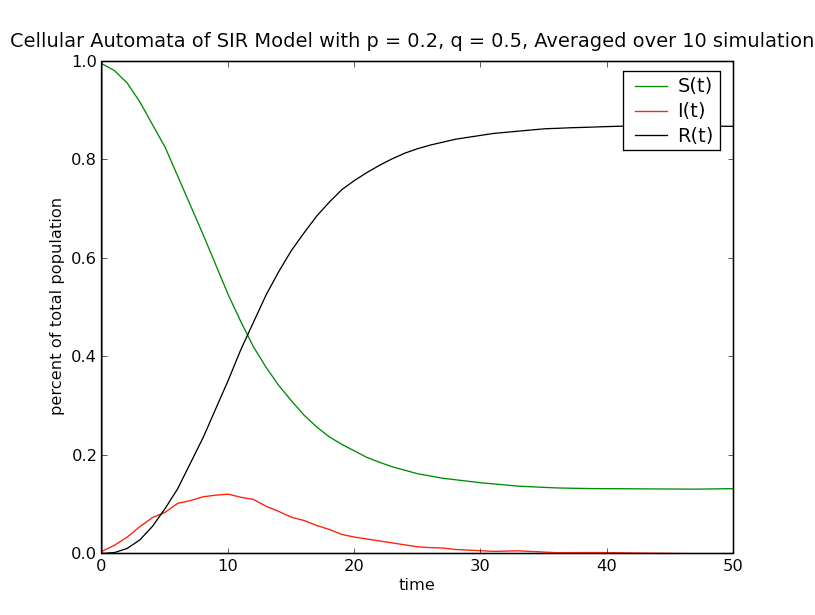
\includegraphics[scale=0.5]{../images/automate_cellulaire_comp.png} 

Ci-dessus sont présentés les résultats d'une autre étude avec un automate cellulaire, il apparaît clairement que leurs courbes sont similaires aux nôtres.

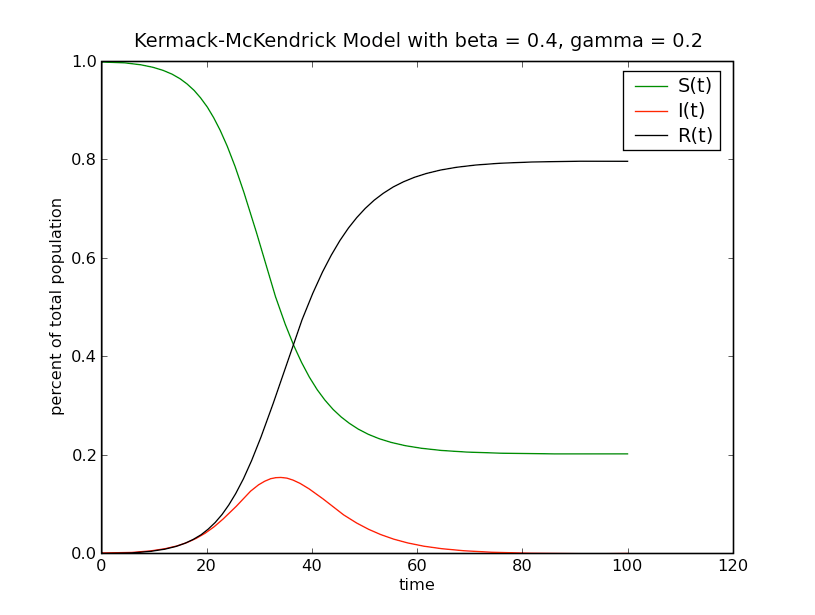
\includegraphics[scale=0.5]{../images/differentiel_1.png} 

De même, les résultats d'une autre étude utilisant la méthode différentielle concordent également à ceux que nous obtenons.

\section{Méthode différentielle}
\subsection{Équations}
	On peut aussi simuler les épidémies par la méthode différentielle. Nous nous sommes basés sur le modèle SIR, c'est à dire le modèle sains, infectés, rétablis. Les équations sont les suivantes :\\
	\begin{align}
		&\frac{dS(t)}{dt} = - \beta I(t)S(t) \\
		&\frac{dI(t)}{dt} = \beta S(t)I(t) - \gamma I(t) - \delta I(t) \\
		&\frac{dM(t)}{dt} = \delta I(t) \\
		&\frac{dG(t)}{dt} = \gamma I(t)
	\end{align}
	
	Ces équations différentielles, une fois résolues, donnent des courbes d'évolution des populations que nous présenterons plus tard.\\
	On remarque notamment que en sommant les quatre équations vues plus haut, on obtient $0$, ce qui semble logique car la population au sens large(incluant les morts) ne varie pas.

\subsection{Propriétés}
	On réintroduit ici les paramètres de la maladie que nous avons défini plus haut, à savoir $R_0$ le taux de reproduction de la maladie, $\tau$ le temps moyen d'infection et $x_0$ la population initiale saine. On pose aussi $\rho = \frac{\gamma}{\beta}$. On a alors $R_0 = \frac{x_0}{\rho}$ 

\section{Appendice}
	\subsection{Code}

\lstset{
  literate=
  {á}{{\'a}}1 {é}{{\'e}}1 {í}{{\'i}}1 {ó}{{\'o}}1 {ú}{{\'u}}1
  {Á}{{\'A}}1 {É}{{\'E}}1 {Í}{{\'I}}1 {Ó}{{\'O}}1 {Ú}{{\'U}}1
  {à}{{\`a}}1 {è}{{\`e}}1 {ì}{{\`i}}1 {ò}{{\`o}}1 {ù}{{\`u}}1
  {À}{{\`A}}1 {È}{{\'E}}1 {Ì}{{\`I}}1 {Ò}{{\`O}}1 {Ù}{{\`U}}1
  {ä}{{\"a}}1 {ë}{{\"e}}1 {ï}{{\"i}}1 {ö}{{\"o}}1 {ü}{{\"u}}1
  {Ä}{{\"A}}1 {Ë}{{\"E}}1 {Ï}{{\"I}}1 {Ö}{{\"O}}1 {Ü}{{\"U}}1
  {â}{{\^a}}1 {ê}{{\^e}}1 {î}{{\^i}}1 {ô}{{\^o}}1 {û}{{\^u}}1
  {Â}{{\^A}}1 {Ê}{{\^E}}1 {Î}{{\^I}}1 {Ô}{{\^O}}1 {Û}{{\^U}}1
  {œ}{{\oe}}1 {Œ}{{\OE}}1 {æ}{{\ae}}1 {Æ}{{\AE}}1 {ß}{{\ss}}1
  {ű}{{\H{u}}}1 {Ű}{{\H{U}}}1 {ő}{{\H{o}}}1 {Ő}{{\H{O}}}1
  {ç}{{\c c}}1 {Ç}{{\c C}}1 {ø}{{\o}}1 {å}{{\r a}}1 {Å}{{\r A}}1
  {€}{{\EUR}}1 {£}{{\pounds}}1
}
\lstset{breaklines=true}

\lstinputlisting[inputencoding=latin1, language=Python]{../tipe_en_cours.py}

\lstinputlisting[inputencoding=latin1, language=Python]{../classes.py}



\newpage

\paragraph{Commentaire bibliographique\\}
\noindent
\cite{ref1} : Cet article nous a permis de bien comprendre la théorie des automates cellulaires, et de mettre l'accent sur les paramètres intéressants qu'une simulation par automate cellulaires permettait de prendre en compte. Il présente aussi les principaux avantages des automates cellulaires par rapport à la méthode différentielle.

\cite{ref2} : Cet article, en plus de présenter un autre modèle d'automates cellulaires, fourni une liste relativement exhaustive de paramètres à prendre en compte dans la simulation(même si les auteurs en ont négligé une partie qui ne présentait qu'un  intérêt minime.

\cite{ref3} : Cet article présente plus en profondeur les différences des autres méthodes,  et fournit une approche intéressante en matière de résultats et de leur présentation.

\cite{ref4} : Cet article présente la méthode différentielle, et est très fourni en graphiques bien expliqués.

\cite{ref5} : Ce livre nous a fournit des éléments sur l'histoire de l'épidémiologie.

\bibliographystyle{plain}

\bibliography{bibliographie}

\end{document}